\documentclass[border=10pt]{standalone}

\usepackage{tikz}
\usepackage{tikzsymbols}
\usetikzlibrary{calc,patterns,shapes.geometric}

\def\centerarc[#1](#2)(#3:#4:#5){\draw[#1] ($(#2)+({#5*cos(#3)},{#5*sin(#3)})$) arc (#3:#4:#5);}

\begin{document}
	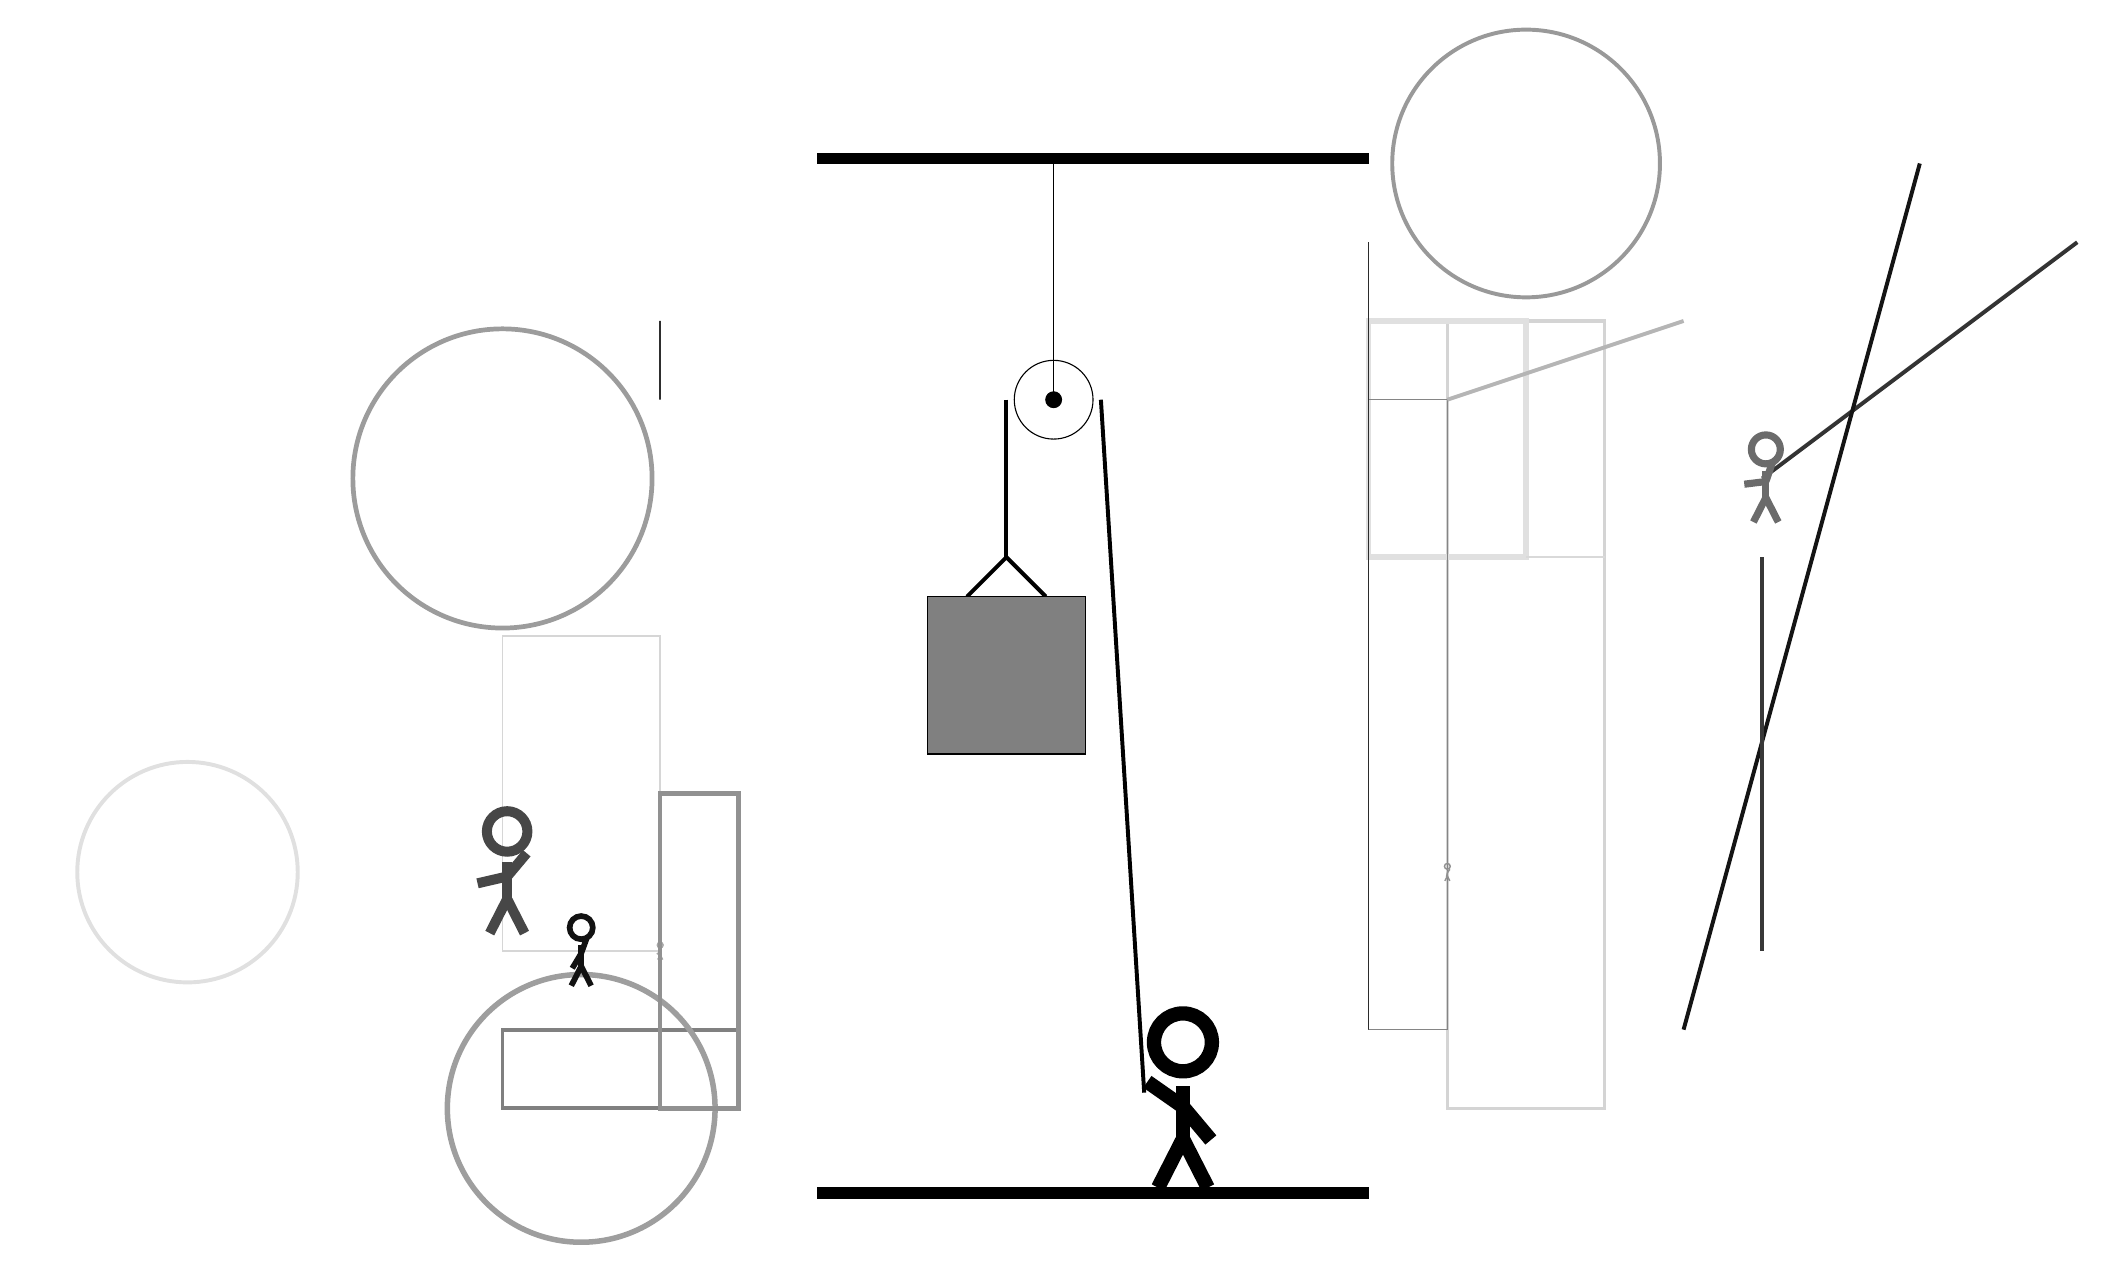
\begin{tikzpicture}
		%%%%% START %%%%%
		
		\draw[fill=black] (-2, 10) rectangle (5, 10.125);
		
		\draw (1, 7) circle (0.5);
		\draw[fill=black] (1, 7) circle (0.1);
		\draw (1, 10) -- (1, 7);
		
		\draw[line width=0.2mm, color=black!16] (-4, 4) rectangle (-6, 0);
		
		\draw[line width=0.3mm, color=black!82] (-4, 7) rectangle (-4, 8);
		\draw [line width=0.6mm, color=black!39](-6, 6) circle (1.9);
		\draw[line width=0.5mm, color=black!80](10, 6) -- (14, 9);
		
		\draw [line width=0.5mm, color=black!40](7, 10) circle (1.7);
		\draw[line width=0.5mm, color=black!92](9, -1) -- (12, 10);
		
		\node[line width=0.7mm, color=black!72] at (-6, 1) {\Strichmaxerl[7][13][50]};
		
		\node[line width=0.5mm, color=black!35] at (-4, 0) {\Strichmaxerl[1][38][76]};
		\draw[line width=0.4mm, color=black!17] (6, -2) rectangle (8, 8);
		\draw[line width=0.5mm, color=black!50] (-3, -1) rectangle (-6, -2);
		\draw [line width=0.5mm, color=black!12](-10, 1) circle (1.4);
		\draw [line width=0.7mm, color=black!38](-5, -2) circle (1.7);
		\draw[line width=0.7mm, color=black!12] (7, 8) rectangle (5, 5);
		
		\draw[line width=0.2mm, color=black!48] (5, -1) rectangle (6, 7);
		\draw[line width=0.6mm, color=black!43] (-3, -2) rectangle (-4, 2);
		\draw[line width=0.2mm, color=black!83] (5, 9) rectangle (5, -1);
		\draw[line width=0.3mm, color=black!15] (7, 5) rectangle (8, 5);
		
		\node[line width=0.3mm, color=black!93] at (-5, 0) {\Strichmaxerl[4][59][70]};
		\node[line width=0.3mm, color=black!58] at (10, 6) {\Strichmaxerl[5][7][71]};
		\draw[line width=0.5mm, color=black!24](5, 9) -- (5, 9);
		\draw[line width=0.5mm, color=black!29](6, 7) -- (9, 8);
		
		\node[line width=0.5mm, color=black!43] at (6, 1) {\Strichmaxerl[1][78][54]};
		
		\draw[line width=0.5mm, color=black!78](10, 0) -- (10, 5);
		\draw [line width=0.6mm, color=black!26](-12, 8) circle (0.0);
		
		\draw[line width=0.5mm] (-0.1, 4.5) -- (0.4, 5.0) -- (0.9, 4.5);
		\draw[fill=black!50] (-0.6, 4.5) rectangle (1.4, 2.5);
		
		\draw[line width=0.5mm] (0.4, 7) -- (0.4, 5.0);
		\centerarc[line width=0.5mm](1, 7)(0:180:0.6);
		\draw[line width=0.5mm](1.6, 7) -- (2.15, -1.8);
		
		\node at (2.6, -1.9) {\Strichmaxerl[10][-35][-50]};
		
		\draw[fill=black] (-2, -3) rectangle (5, -3.15);
		
		%%%%% END %%%%%
	\end{tikzpicture}
\end{document}